
%\subsection{Introduction}







%===================================================The aim of this paper===============================================
%We first provide an overview of state-of-the-art API and third-party library recommenders, discussing  how they could be potentially affected by AML.

%Through a literature search from premier venues in Software Engineering for adversarial techniques, I show that there are considerably evident threats to RSSE. 
%Then, we perform a preliminary examination of two existing systems for recommending third-party libraries. The experimental results reveal a worrying outcome: by a simple manipulation, we can seamlessly spoil the final recommendations, putting software clients at risk.

%In this section, we present the proposed approach.

%The prospective work is not a fresh %completely new 
%start, but a continuation of our current research presented in Section~\ref{sec:CurrentResults}. %Our focus is to find methods to defuse popularity bias, and deal with adversarial attacks. 


%The research aims to contribute to the resilience and trustworthiness of recommender systems used in software engineering contexts, ultimately safeguarding users and valuable software assets. 
Figure~\ref{fig:SystemArchitecture} depicts the architecture with the proposed module printed in the cyan color, which can be independently assembled to any existing recomender systems %. The first module is used to detect and eliminate adversarial intents disguised in the training data, meanwhile, the second module is 
%being padded right before the interface to developers 
to defuse popularity bias.
This section presents our proposed approach to fill the research gap introduced in Section~\ref{sec:Introduction}. %, before presenting the results.



%\subsection{Adversarial attacks}

%\section{Project overview}

%\section{Background}
% \cite{Dagenais:2010:MNS:1806799.1806842} (often at a short time)

%Deep learning techniques exploit multiple layers to better capture features from an input and.
%Deep Neural Networks architectures are designed 
% where every single layer only receives a connection from previous and provides connections only to the next layer in the hidden part
%The implementation of Deep Neural Network (DNN) is basically a discriminatively trained model that uses the standard back-propagation algorithm and sigmoid or ReLU as activation functions. 
%assigns more weights to the previous data points of sequence. Therefore, this technique is 
%can be used for text mining and classification. 
%considers the information of previous nodes in a very sophisticated method which 
%Deep learning is a technique that allows computational models composed of multiple processing layers 

%In the domain of Mining Software Repositories (MSR), 
%the ultimate aim is to discover serendipitous relationships among open source software projects by analyzing the rich data available in software repositories. In software repositories, the volume of data grows exponentially and turns to be increasingly inconsistent over the course of time. At the expense of the data model, data accessing and processing appears to be a daunting task. This makes the cost for maintaining information integrity become prohibitive. The requirement of knowledge sharing and interoperability necessitates an adequate modeling of diverse software artifacts, e.g., issue tracker, version tracker. Given the heterogeneity and constant changes of the underlying distributed data in MSR, the utilization of XML and databases is not sufficient for fulfilling the above mentioned requirements. Furthermore, the lack of a common format in software repositories makes it difficult to integrate data from various sources to produce recommendations as well as to forecast project evolution. To this end, a uniform knowledge base that facilitates data representation and integration is of highly importance. The knowledge base is expected to render possible innovative features and enable the discovery of useful or interesting relationships by chance. Based on this representation, it is then possible to detect project incompatibilities and to identify complementary and competing projects. 

%I propose conducting a prospective research which is going to be based on three core research theme: \emph{Mining OSS Repositories}, \emph{Recommender Systems}, and \emph{Deep Learning}. 
%In this sense, DNN exploit the standard back-propagation algorithm and sigmoid or a rectified linear unit (ReLU) as the activation function. Several deep neural network architectures have been proposed to increase both prediction accuracy and efficiency. 
%The ability to . 
%and from existing data by 
%To integrate various types of recommendations. 

%Conventional neural networks connect all the neurons of a layer to the next layer, and the number of weights increases over the number of layers. 

%For building and 
% the capability
%into 
%First, it is necessary to provide developers with instant recommendations. The re that best fit their needs. 
%This is done 
%assign more weights to the previous data points of sequence. An RNN 

%===================================
%An LCD platform needs to be equipped with built-in modules offering various functionalities, which can be instantly embedded whenever developers drag and drop them into their working panel. Such modules are provided by mining OSS repositories to integrate different types of recommendations. To this end, I plan to investigate and deploy suitable recommender systems to supply different artifacts, \eg source code, API usage patterns, third-party libraries. Furthermore, I am going to study the feasibility of applying DNNs to generate recommendations, \eg source code classification, software size estimation, automatic software repair, API sequences, to name a few. For instance, Recurrent Neural Networks (RNNs) are a family of neural network architectures that allow for better semantic analysis of the structures in a dataset, thereby being highly suitable for the classification of textual and sequential data. RNNs can be used to classify software systems by means of source code, or to classify API documentation. Still, the identification of suitable DNNs for mining OSS repositories is dependent on a more detailed investigation. 

%clustering open source software projects 
%In this sense, I am going to investigate in detail the suitability of.

%\vspace{-.3cm}

\begin{figure}[h!]
	\centering
	%	\vspace{-.2cm}
	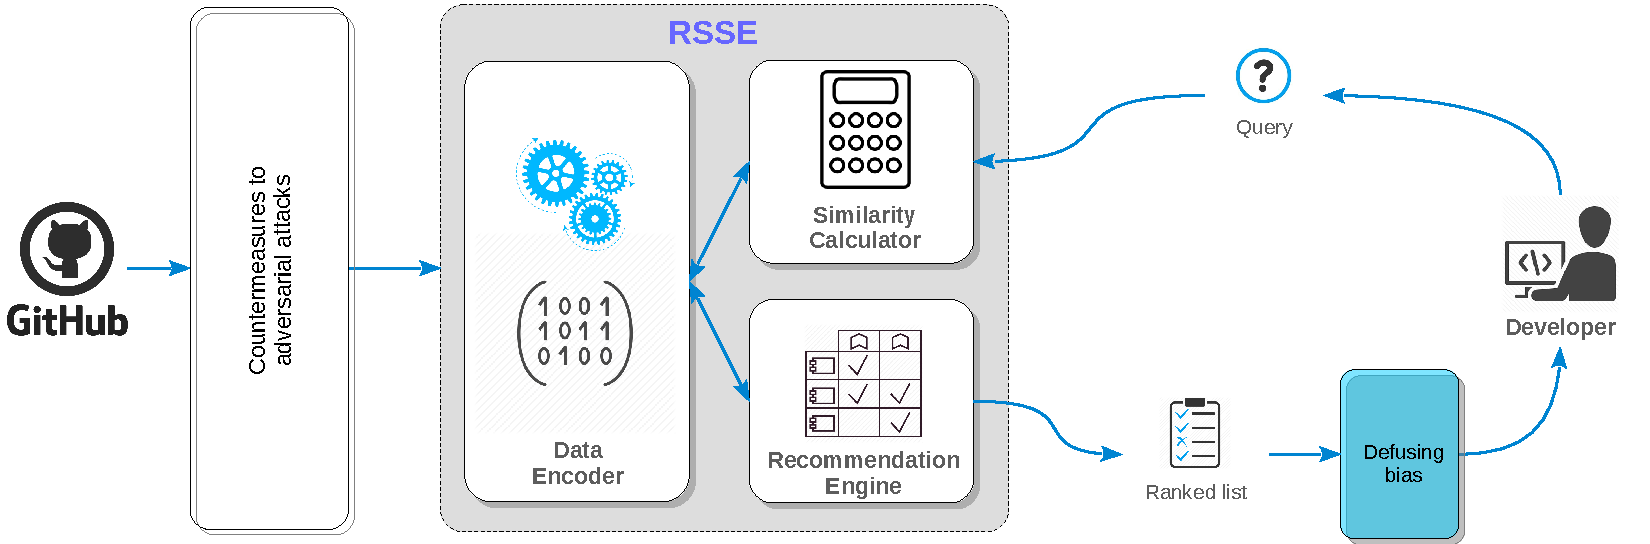
\includegraphics[width=0.60\columnwidth]{figs/SystemArchitecture.pdf}
	\vspace{-.2cm}
	\caption{The proposed architecture.}
	\vspace{-.4cm}
	\label{fig:SystemArchitecture}
\end{figure}


%=================================
%\begin{figure}[h!]
%	\centering
%	%	\vspace{-.2cm}
%	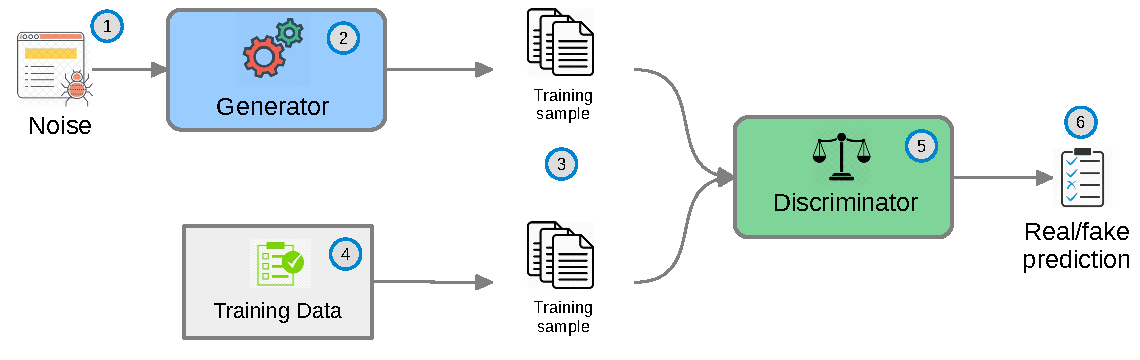
\includegraphics[width=0.60\columnwidth]{figs/GAN.pdf}
%	\vspace{-.2cm}
%	\caption{Architecture of a Generative Adversarial Network~\cite{DBLP:journals/csur/WangSW21}.}
%	%	\vspace{-.3cm}
%	\label{fig:GAN}
%\end{figure}
%=================================






\subsection{Research objectives}




%	\item a machine learning model to protect privacy in software engineering systems.
%	\item Users are reluctant to share their data.
%	\item Machine learning models tailored to software engineering applications.

%Within the project funded by Sony, 
%In particular, 

%We are going to conceptualize suitable techniques for building %address the related issues 
%fair and robust recommender systems for Software Engineering by 

%To be concrete, 
%Correspondingly, 
Within the funded project, we are going to answer the following research questions.

%The present paper makes the following contributions: 
%\begin{itemize}
%	%	\noindent
%	\item[--] A discussion on the possible adversarial attacks to state-of-the-art RSSE for third-party libraries and API calls; 
%	\item[--] A preliminary evaluation on two library recommender systems to perturb their recommendations.
%\end{itemize}

\begin{itemize}

	\item[--] \textbf{RQ}: ``\emph{How can we make RSSEs less biased towards popular items, while still preserving accuracy?}'' We plan to develop novel methods to defuse popularity bias. Existing mechanisms conceived for other domains might not work well for recommender systems for software engineering, as we showed in our recent work~\cite{10174041}. We anticipate that Reinforcement Learning~\cite{DBLP:books/lib/SuttonB98} can be applied to improve re-ranking techniques, taking into consideration the similarity between projects when a rare library needs to be moved up in the ranked list. %the libraries that need to re-ranked, and the ones that contain.	
	
%	\item[--] \textbf{RQ2}: ``\emph{How can we defend RSSEs against adversarial attacks?}'' Given the existing threats, it is necessary to conceive effective countermeasures that can ward off attacks tailored to RSSE. This is done by studying learning algorithms being aware of adversarial attacks and seize them. Moreover, adversarial attempts should be turned into features for the 
%	training process, \ie RSSEs should not only learn from useful patterns, but also be able to learn how to avoid hostile patterns.
\end{itemize}

%, while allowing 
%Our work reveals that software engineering research has not properly dealt with popularity bias in TPL RSSEs, triggering the need for effective counteracting mechanisms. %Looking at other domains, 
%we see that there are three major methods to combat bias in general, \ie the pre-processing, in-processing, and post-processing paradigms~\cite{doi:10.1089/big.2016.0048}. We assume that they can also be adopted in Software Engineering for the same purpose, as it was also advocated by Chakraborty \etal \cite{ChakrabortyM0M20}, though not directly for RSSEs. %Also, as it can be seen from Section~\ref{sec:Results}, He \etal~\cite{9043686} conceived 
%\LS~\cite{9043686} is the very first TPL RSSE to mitigate the abundance of highly frequent libraries, following the \emph{in-processing} approach. \LS attempts to neutralize the bias caused by the popularity of TPLs using an adaptive weighting mechanism. However, while it can diversify the recommendations, \LS suffers from a low accuracy (see RQ2 in Section~\ref{sec:RQ2}). This implies that there is still room for improvement, \ie conceiving more effective in-processing techniques for RSSEs.


To answer the research question, correspondingly we divide the activities into three tasks, namely \textbf{T1}, \textbf{T2}, and \textbf{T3}, % (see Figure~\ref{fig:SystemArchitecture}), %and they are 
explained in the succeeding subsection.
%\vspace{-.4cm}






\subsection{Defusing popularity bias}


Our research~\cite{10174041} reveals that software engineering research has not properly tackled popularity bias in RSSEs, triggering the need for effective counteracting mechanisms. 
Looking at other domains, we see that there are three major methods to combat bias, \ie the pre-processing, in-processing, and post-processing paradigms~\cite{doi:10.1089/big.2016.0048}. We assume that they can also be adopted in Software Engineering for the same purpose, as it was advocated by Chakraborty \etal \cite{ChakrabortyM0M20}, though not directly for RSSEs. Moreover, we anticipate that reinforcement learning and self-improvement learning can be employed to defuse bias, bringing more diverse recommendation results. In this respect, our proposal is going to be based on three main topics as follows.
%Also, as it can be seen from Section~\ref{sec:Results}, He \etal~\cite{9043686} conceived \LS--the very first TPL RSSE to mitigate the abundance of highly frequent libraries, following the \emph{in-processing} approach. \LS attempts to neutralize the bias caused by the popularity of TPLs using an adaptive weighting mechanism. However, while it can diversify the recommendations, \LS suffers from a low accuracy (see RQ$_2$ in Section~\ref{sec:RQ2}). This implies that there is still room for improvement, \ie conceiving more effective in-processing techniques for RSSEs. 

%Our work~\cite{10174041} reveals that the issue of popularity bias in RSSEs has not attracted attention from the research community, triggering the need for effective counteracting mechanisms. 
%The application of various Machine Learning algorithms to tackle bias in RSSEs.
%Looking to other domains, we see that there are three major methods to defuse bias in general, \ie the pre-processing, in-processing, and post-processing paradigms~\cite{doi:10.1089/big.2016.0048}. Our proposed approach is based on three main techniques, \ie .
%We suppose that these can also be adopted in software engineering for the same purpose. %as it was also advocated by Chakraborty \etal \cite{ChakrabortyM0M20}, though not directly for RSSEs. 
%We are going to perform the following tasks:

\begin{itemize}
	\item \textbf{T1: Re-implementation of existing re-ranking mechanisms.} In our recent work~\cite{10174041}, we applied xQuAD \cite{10.1145/1772690.1772780} %--an algorithm for diversifying Web search results, 
%	and the technique allowed us 
	to improve diversity in the recommendations. %Nevertheless, such the improvement is marginal, and there exists a light setback in accuracy. 
	We plan to investigate and re-implement other %re-ranking 
	techniques, with the aim of finding suitable mechanisms to be adopted for RSSEs. Another possible candidate is PFAR~\cite{DBLP:journals/corr/abs-1809-02921}, a practical approach conceived to allow items to have a fair chance of being recommended. We will considered also personalized ranking~\cite{DBLP:conf/flairs/AbdollahpouriBM19}, which promotes unpopular items in the ranked list, while maintaining a trade off between fairness and accuracy. Once re-implemented, these techniques can be used as baselines for comparison with our proposed approach presented in \textbf{T2}. %as well as to i%Thus, it is necessary. 
%, \eg the frequency of occurrences may. %, \eg r.
%\emph{Pre-processing} techniques can also be useful for TPL RSSEs, \eg by considering factors related to peculiar, solution-specific aspects of a project that, as pointed out in Section \ref{sec:Background} are neglected, and that would help reward certain libraries. From RQ1, we see that no approach specifically employs pre-processing to cope with popularity bias in RSSEs.
	\item \textbf{T2: Reinforcement learning for reducing bias.} Existing re-ranking algorithms such as xQuAD~\cite{10.1145/1772690.1772780} %rearrange the recommendation lists, aiming 
	attempt to reduce the number of popular items, as well as to increase the number of unpopular (but useful) ones in the results. However, our empirical evaluation on two recommender systems showed that while introducing diversity in the recommendation results, it also introduces a setback in the prediction accuracy. Our findings suggest that %Software Engineering 
	further research should be conducted to propose effective countermeasures. We suppose that it is crucial to consider %further improve it by considering 
	additional factors, \eg the degree of specificity (to certain solutions) of a library, when it comes to providing recommendation. Thus, we will deploy Reinforcement Learning to implement effective post-processing techniques to defuse popularity bias, aiming to improve diversity in the recommendations, while keeping a reasonable prediction accuracy. % without touching the internal design of the considered systems.
	\item \textbf{T3: Self-improvement learning for improving ranking.} %Recently, various algorithms have been proposed to improve the learning processing. 
	Self-improvement learning allows a model to incorporate its own predictions into the training process~\cite{wang2020exposure}. This enables the model learn from its errors, thereby lessening the effects of exposure bias. Such an algorithm can be applied to improve ranking of items provided by a recommender system. In particular, we train the model with collected training data, and once the model has been trained, it is used to generate for each sample in the training dataset a set of predictions. For each training sample, we compute the diversity scores between the ground-truth list and all the predictions. The predicted libraries with the highest diversity is then chosen to replace the ground-truth one. We get a new training pair composed of the input sample, and the new ground-truth library. By replicating the steps with all the training samples, we get the so-called augmented training dataset that can then be used to re-train the model.

	% ...%The technique is built 
%Starting from an initial ranked list $R$, we look for the long-tail items in the list, and promote them to upper positions to yield a new list $S$. %We call %$R$ as the list provided by a recommender, and 
%$S$ is initially set to $\varnothing$, and iteratively populated by enrolling new items using the following formula.
%	\item The result of this workpackage is Deliverable \textbf{D1}: ``\emph{Defusing popularity bias with reinforcement learning}.''
\end{itemize}
\vspace{-.4cm}





%\subsection{WP2: Generating malicious data; Adversarial training}
%
%%Generative Adversarial Networks
% 
% \begin{itemize}
%	\item[--] \textbf{T2.1: Generating fake data with GANs.} %\textbf{RQ2}: ``\emph{Can GAN cause threats to third-party library and APIs recommender systems?}'' 
%%We plan to study the threats that cause harm or danger to RSSE suggesting third-party libraries and API function calls. %These two types of recommendations have been selected as they are representative scenarios in which \emph{(i)} the recommendation is learned from OSS repositories; and \emph{(ii)} the outcome of a malicious recommendation, \eg the usage of a library or an API, can cause troubles to end-users.%result in severe security holes.%~\cite{10.1145/2976749.2978333}.
%To defend a system against attacks, it is necessary to be knowledgeable of various types of adversary activities~\cite{4216981}, which generate perturbations to deceive and disrupt systems by %causing a malfunction, 
%compromising their recommendation capabilities. 
%%A main way to achieve this is to feed systems with malicious data~\cite{DDM20a}.
%The ultimate aim of these attacks is to manipulate target items, thus creating  either a negative or positive influence on the final recommendations~\cite{10.1007/s10462-012-9364-9}, depending on the attacker's 
%intention. %For instance, in image classification, an attacker crafts an input image by adding non-random noise in a way that it will be imperceptible to ML models, whilst still being properly recognized by 
%%humans~\cite{conf/cvpr/NguyenYC15}. As an example, a panda was recognized as a ribbon by cutting-edge deep neural networks once the input image had been padded with noise, meanwhile humans still correctly perceived the panda from the forged image~\cite{DBLP:journals/corr/GoodfellowSS14}.
%Generative Adversarial Networks \cite{10.5555/2969033.2969125} (GANs) have been widely used in image processing to produce crafted images, which resemble real ones. %are a very popular class of deep generative models which have shown some incredible results in generating images. 
%GANs consist of two main components, \ie Generator and Discriminator. Generator is a deep neural network and accepts as input both real training data and crafted data, \ie noise. %is trained to take a random input $z$.
%%The idea behind GANs is to train two networks simultaneously. 
%%Firstly, a generator network, which we can train to take a random input (often called  z) and produce a sample from some distribution, in this case, the distribution of 28 $\times$ 28 grayscale clothing images. 
%Discriminator is also a deep neural network and it learns to distinguish the real training data from the crated data, to provide the final prediction. In other words, Generator is trained with real and forged data to trick Discriminator, which in turns attempts to avoid being tricked by learning from real training data.
%According to our investigation, GANs can also be exploited to generate fake training data to feed RSSEs. %This section briefly recalls the main technical details of GANs.\footnote{The background of GANs as well as the corresponding notions originate from \url{https://bit.ly/3hizVtf}} %Deep neural networks have been exploited to generate perturbations.  
%We suppose that GANs can be used to produce crated training OSS projects to compromise RSSEs. In this respect, it is necessary to perform a detailed investigation on this topic, as well as to find effective countermeasures that can deal with this type of adversarial attempts.

%	\item[--] \textbf{T2.2: Anomaly detection and adversarial training.} To mitigate the impact of ill intents to recommender systems, anomaly detection techniques can be considered as a viable strategy. This involves identifying malicious API patterns before they are recommended to developers. For instance, a statistical process control strategy~\cite{10.1145/1097047.1097061}, has proven effective in recognizing suspicious items by assessing two critical parameters: the distribution density of items and their average ratings. For RSSEs, detecting anomalies corresponds to the distribution patterns of APIs within software projects and declarations. %However, it is imperative to approach this task with care to minimize the risk of false positives and false negatives. 
%API distributions can span a wide spectrum, covering not only extremely popular APIs but also rare and less common ones. Therefore, relying solely on radical patterns, such as those that are excessively popular or exceedingly rare, may not guarantee successful discrimination in all cases. A more tailored approach involves the detection of malicious and benign API sequences by monitoring a specific set of third-party libraries with supervised classifiers~\cite{10.1109/COMPSAC.2015.241}. While this approach holds promise, it does not come without limitations, \ie it may perform well in detecting malicious sequences comprised of APIs from a predefined set of libraries, but may not be universally applicable to patterns containing only a few APIs sourced from less popular libraries. %, warranting further exploration and refinement.
%	\item[--] The results of this workpackage is Deliverable \textbf{D2}: Dealing with fake data using adversarial training.
%
%\end{itemize}


%========================
%Figure~\ref{fig:GAN} illustrates a GAN which consists of two main components, namely Generator and Discriminator. Generator \circled{2} is a deep neural network and accepts as input both real training data \circled{4} and crafted data \circled{1}, \ie noise. %is trained to take a random input $z$.
%%The idea behind GANs is to train two networks simultaneously. 
%%Firstly, a generator network, which we can train to take a random input (often called  z) and produce a sample from some distribution, in this case, the distribution of 28 $\times$ 28 grayscale clothing images. 
%Discriminator \circled{5} is also a deep neural network and it learns to distinguish the real training data from the crated data, to provide the final prediction \circled{6}. In other words, Generator is trained with real and forged data to trick Discriminator, which in turns attempts to avoid being tricked by learning from real training data. %This process is described in the following diagram:
%
%
%%The main idea is to train the generator with and discriminator, by minimizing the. 
%%(one that makes the fewest mistakes possible) 
%% Of course, in practice, we do not necessarily have an optimal discriminator, and so we end up with some approximation of the JSD.
%%Let's take a closer look at what the JSD is and how it is approximated.
%%We can, and will in just a moment, prove that 
%%https://colab.research.google.com/github/khipu-ai/practicals-2019/blob/master/3b_generative_models.ipynb#scrollTo=5f0u8t0K5FOk
%
%In this context, Discriminator plays the role of a loss/error function to train Generator. %by approximating the Jensen-Shannon divergence (JSD). 
%Using Discriminator to train Generator boils down to minimizing the JS-divergence between the distributions of the generated and real data. The final aim is to minimize the loss, which is defined using the following formula \cite{10.5555/2969033.2969125}:
%
%%In this respect, Jensen-Shannon Divergence (JSD) is used to measure the similarity between two probability distributions. 
%
%\begin{equation} \label{eqn:loss1}
%	E_{x\sim p_{d}(x)}\left [ log D^{*}(x)\right ] + E_{z\sim p_{z}(z)}\left [ log(1-D^{*}(G(z)))\right ]
%\end{equation}
%
%%from which we draw samples to pass through our generator
%%\vspace{-.2cm}
%$D^{*}(x)$ is defined as follows:
%\begin{equation} \label{eqn:D}
%	D^{*}(x) = \frac{p_{d}(x)}{p_{d}(x)+p_{g}(x)}
%\end{equation}
%
%where $p_{d}(x)$ is the distribution of the training data, and $p_{z}(x)$  is the distribution of the noise. 
%
%The first component, \ie $E_{x\sim p_{d}(x)}\left [ log D^{*}(x)\right ]$ corresponds to attempts to recognize real data better, while the second component, \ie $E_{z\sim p_{z}(z)}\left[ log(1-D^{*}(G(z)))\right ]$ means that the engine can spot fake data better.
%========================





%By substituting Eq.~\ref{eqn:D} into Eq.~\ref{eqn:loss1}, we get the following equation.
%\begin{equation}
%E_{x\sim p_{d}(x)\left [ log D^{*}(x)\right ]} + E_{z\sim p_{z}(z)\left [ log(1-D^{*}(G(z)))\right ]}
%\end{equation}
%\vspace{.2cm}





%	\item  









%
%\subsection{WP2: Countermeasures to adversarial attacks}
%
%
%To equip RSSEs with robust defense mechanisms against malicious endeavors, we are committed to developing innovative techniques to identify and thwart malicious APIs. Additionally, we acknowledge the significance of adversarial training, \ie training machine learning models on manipulated data to enable them to discern adversarial intent from benign ones. %To this end, 
%Our research will focus on the following key tasks:%key aspects:
%
%%To equip RSSEs with effective mechanisms to defend against hostile attempts, we will develop %countermeasures %. We intend to develop defense mechanisms from the following two perspectives: \emph{(i)} internal view, \ie design of recommender systems; and \emph{(ii)} external view, 
%%techniques to %detect and protect against hostile attempts, %. Concerning the former, we study counteractions conceived for generic recommender systems in the hope of customizing them for RSSE. With the latter, 
%%recognize and seize malicious APIs. Moreover, we also consider adversarial training, \ie training a machine learning model with manipulated data, so as allowing it to learn how to distinguish bad intents from the good ones. In particular, our proposal will be focused on the following aspects:%techniques:
%
%%===========================https://bkai.ai/seminar-adversarial-learning-foundations-and-applications/===========================
%%Adversarial robustness aims to improve the robust accuracy of ML models on adversarial data, which can be achieved by adversarial training (AT). Specifically, AT has two purposes: (1) correctly classify the data (the same as ST) and (2) ensure no data fall nearby the decision boundaries (different from ST). Given that the test data may be adversarial, AT carefully simulates some adversarial attacks during training. Thus, the model has already seen many adversarial training data in the past with the purpose of generalizing to adversarial test data in the wild. 
%%===========================
%%In the following, we discuss possible 
%
%% and protect RSSE. %API recommender systems.%anomaly detection techniques that can be used for API recommenders.
%%Countering adversarial attacks through a
%
%
%\begin{itemize}
%	\item \textbf{T2.1: Mitigating the impact of manipulated projects.} Utilizing model-based algorithms offers a valuable approach for addressing the influence of manipulated profiles within recommender systems, particularly in the context of open-source software (OSS) projects~\cite{4216981}. These algorithms excel in the task of categorizing similar profiles, effectively grouping OSS projects into distinct segments. While these techniques may not provide absolute immunity against malicious projects, their primary goal is to diminish the prevalence of projects exhibiting abnormal behaviors. Such projects should not be categorized as similar to any active or legitimate projects currently under development. This methodology allows us to significantly reduce the likelihood of %recommender 
%	systems selecting and incorporating deceptive or spurious data, thus defending them against from potential attacks. Moreover, this approach can be applied to improve the security of RSSEs relying on similarity, %or collaborative-filtering techniques, 
%	\eg UP-Miner \cite{Wang2013Mining}, MUSE \cite{Moreno:2015:IUT:2818754.2818860}, FOCUS~\cite{Nguyen:2019:FRS:3339505.3339636}, or CodeKernel \cite{DBLP:conf/kbse/Gu0019}. %However, it is worth noting that implementing this method necessitates the thorough redesign of the foundational building blocks of these systems, making it a complex endeavor that may require substantial effort and resources.% to execute effectively.
%
%%	\item \textbf{T2.2: Enhancing resilience through profile classification.} Profile classification can be an effective mechanism in fortifying the resilience of RSSEs against malicious attacks~\cite{10.1145/1097047.1097061}. The process begins by constructing a training dataset that encompasses both authentic projects and synthetic projects generated according to a predefined attack model. To streamline the dataset, attribute-reduction techniques can be applied, reducing the number of features required for representation. Following dataset preparation, supervised classifiers are trained on the refined dataset. The ultimate objective is to distinguish between genuine and synthetic projects, effectively detecting instances where malicious data has been inserted. The efficacy of this technique is enhanced given that an ample volume of training data is available, covering diverse approaches to populating synthetic (fake) projects. We postulate that a multifaceted approach, %implementation of a hybrid security model, 
%%	which aggregates internal and external perspectives, holds significant promise in boosting the robustness and resilience of RSSE against adversarial attacks. Internal countermeasures enable RSSEs to preemptively sidestep falsified data sources, while external-view defense mechanisms facilitate the detection of concealed malicious intent within API patterns before recommending them to developers. %This multifaceted approach serves as a comprehensive shield against potential threats to RSSE integrity.
%	
%	\item \textbf{T2.2: Anomaly detection and adversarial training.} To mitigate the impact of ill intents to recommender systems, anomaly detection techniques can be considered as a viable strategy. This involves identifying malicious API patterns before they are recommended to developers. For instance, a statistical process control strategy~\cite{10.1145/1097047.1097061}, has proven effective in recognizing suspicious items by assessing two critical parameters: the distribution density of items and their average ratings. For RSSEs, detecting anomalies corresponds to the distribution patterns of APIs within software projects and declarations. %However, it is imperative to approach this task with care to minimize the risk of false positives and false negatives. 
%	API distributions can span a wide spectrum, covering not only extremely popular APIs but also rare and less common ones. Therefore, relying solely on radical patterns, such as those that are excessively popular or exceedingly rare, may not guarantee successful discrimination in all cases. A more tailored approach involves the detection of malicious and benign API sequences by monitoring a specific set of third-party libraries with supervised classifiers~\cite{10.1109/COMPSAC.2015.241}. %While this approach holds promise, it does not come without limitations, \ie it may perform well in detecting malicious sequences comprised of APIs from a predefined set of libraries, but may not be universally applicable to patterns containing only a few APIs sourced from less popular libraries. %, warranting further exploration and refinement.
%	\item The result of this workpackage is Deliverables \textbf{D2}: ``\emph{Defending RSSEs against adversarial attacks,}'' and \textbf{D3}: ``\emph{A holistic approach to fairness and robustness of RSSEs}.''%Defending RSSEs against adversarial attacks. %Dealing with adve using adversarial training.
%		
%\end{itemize}
%\vspace{-.4cm}
%%``\emph{}.''
	
%	\item \textbf{Minimizing the effect of manipulated profiles.} Model-based algorithms are of great use as they can be applied to cluster similar profiles (OSS projects) into \emph{aggregate segments}~\cite{mobasher_attacks_2007}. Though these techniques cannot entirely isolate malicious projects, this aims to lessen the prevalence of projects with abnormal behaviors, \ie they will not be seen as similar to any active projects, \ie the ones under development. In this way, such a method reduces the possibility that RSSE select and incorporate bogus data, thereby avoiding attacks. The method can be applied to defend RSSE that work based on a similarity or collaborative-filtering technique, such as UP-Miner \cite{Wang2013Mining}, MUSE \cite{Moreno:2015:IUT:2818754.2818860}, FOCUS~\cite{Nguyen:2019:FRS:3339505.3339636}, or CodeKernel \cite{DBLP:conf/kbse/Gu0019}. Nevertheless, it requires the redesign of the whole systems' underpinning building blocks, and thus, it is not easy to conduct.  %Furthermore, it may not be applicable to other systems, such as MUSE, or.
%	\item Adversarial attacks can be counteracted using \textbf{anomaly detection techniques}, \ie recognizing malicious API patterns before they are recommended to developers. %There have been approaches conceived to detect malicious API sequences. 
%	For instance, a statistical process control strategy~\cite{mobasher_attacks_2007} has been used to identify suspicious items by examining two parameters, namely items' distribution density and average ratings. By referring to RSSE, we can think of detecting anomalies from the distributions of APIs in projects and declarations. This, however, necessitates careful analyses to avoid false positives and false negatives. %As shown in Section~\ref{sec:rq2-design}, 
%	The distributions of APIs may span in a wide range, \ie there are not only extremely popular APIs but also rare ones. Thus, being based on a radical pattern, \eg a too popular or too rare one, the detection of malicious APIs may not succeed in every case. A more tailored approach is to tell malicious/benign API sequences apart by monitoring a certain set of third-party libraries using supervised classifiers~\cite{10.1109/COMPSAC.2015.241}. Such an approach, however, has its limitation as follows. Though it can detect malicious sequences consisting of APIs from a specific set of libraries, it may not be applicable to patterns with a few APIs coming from a less popular library.
%	\item \textbf{Profile classification} can also help increase the resilience of RSSE against malicious attacks~\cite{10.1145/1097047.1097061}. First, it is necessary to build a training set consisting of both authentic projects and fake projects that are generated following an attack model. Attribute-reduction techniques may be used to reduce the number of features needed to represent the dataset. Afterward, supervised classifiers are trained on the resulting dataset to classify real and fake projects, aiming to detect the injection of malicious data. This technique works more effectively when we have enough training data by taking into consideration different ways of populating fake projects. In conclusion, we believe that a hybrid security model, consisting of countermeasures pertaining to both an internal (design) and external view, is likely to contribute to the robustness and resilience of RSSE towards adversarial attacks. While internal countermeasures allow RSSE to avoid falsified or suspicious data sources, defense mechanisms based on external view help RSSE detect malicious intent hidden in API patterns before recommending them to developers.%, RSSE may check for its eligibility.

%\UM~\cite{Wang2013Mining}, PAM~\cite{Fowkes:2016:PPA:2950290.2950319}, and \FC~\cite{Nguyen:2019:FRS:3339505.3339636}



%I am going to conduct an evaluation on two library recommender systems to perturb their recommendations. 






